\section{Recorded Time, Configuration, and Additional Costs}
\label{app:resource-details}
\suppressfloats[t]
This appendix records worker usage, historical preparation, and supporting sessions. Call receipts, controller records, and session logs supply the values. The extracts \path{evidence/timing-model-audit.json}, \path{evidence/support-session-usage.json}, and \path{evidence/accounting-and-release.json} retain the inputs, intervals, hashes, and release decisions.

\paragraph{Recorded configuration}
The 117 receipts record requests for \texttt{gpt-6-astra}. They identify the same Codex client binary, version 0.155.1. The SNG worker matches its frozen source hash. Its options include \path{--strict-config}, \path{--ignore-user-config}, \path{--ignore-rules}, and \path{--ephemeral}. It uses a temporary configuration directory and a JSON output schema. Appendix~\ref{app:evaluation-details} identifies the Sireum and cvc5 versions.

\paragraph{Intervals in the main evaluation}
Table~\ref{tab:recorded-timing} gives dispatch, check, and elapsed times. On 6 November 2026, SNG $K^{+}$ started at 07:49:38.630693 UTC. Observation ended at 10:20:59.935633 UTC. The difference is 9,081.305 seconds, or 2\,h 31\,min 21.3\,s. It spans the initial model phase, rejected proposal, authorized repairs, approval pauses, and final observation. Model dispatch across the eight experiment calls totals 1,123.279 seconds (18.72 minutes). The final observation lasts 20.033 seconds after readiness.

Producer/Consumer's separate, unpaired baseline follow-up used 305,087 measured tokens, with 358.59 seconds of model dispatch and checks across a 940.49-second elapsed interval. The interval includes 567.48 seconds of harness recovery and authorization. Each of the two interrupted Producer/Consumer runs retains a separate 1M estimated usage debit~\cite{producerConsumerConsolidatedReport2026}.

\begin{table}[!htbp]
\caption{Measured experiment-model tokens and time in seconds. Dispatch includes call handling. Elapsed time includes interruptions and pauses. SNG milestones are cumulative except for the paid-repair increment. Dashes mark unavailable totals.}
\label{tab:recorded-timing}
\centering\small
\begin{tabular}{@{}p{.40\linewidth}rrrr@{}}
\hline
Recorded point & Tokens & Dispatch & Checks & Elapsed \\
\hline
Later Producer/Consumer $K^{+}$ & 179,515 & 109.53 & 94.45 & 210.19 \\
Later Producer/Consumer $K$, interrupted & 48,236 & 36.35 & 17.40 & 57.86 \\
Later SNG $K$, repair limit & 388,726 & 682.71 & 362.30 & 1,052.77 \\
Later SNG $K^{+}$, model checks & 346,224 & 532.43 & 154.10 & --- \\
SNG $K^{+}$, proposal rejected & 424,693 & 785.67 & 154.10 & 949.80 \\
SNG $K^{+}$, paid repair increment & 151,909 & 337.61 & 280.18 & 627.67 \\
SNG $K^{+}$, through observation & 576,602 & 1,123.28 & --- & 9,081.30 \\
\hline
\end{tabular}
\end{table}

\paragraph{Experiment-worker ledger}
Table~\ref{tab:ledger-scope} in the main evaluation gives the disjoint case totals through SNG closeout. The parent campaign's 67 calls used 3,060,221 measured tokens plus 2M estimated debits under its 6,310,229 ceiling. Fifty earlier calls contribute the remaining 6,256,540 accounted tokens.

A ledger observation at 18:17:25 UTC on 8 November includes 24 later BASS calls, adding 1,382,740 measured tokens. The broader balance then reached 12,699,501 accounted tokens, with a parent ceiling of 7,560,221. Successive BASS reports contain overlapping sets of 14, 19, and 24 calls; the later balance counts the final 24-call set once. The three-case accounting in Table~\ref{tab:ledger-scope} uses the earlier SNG closeout.

\paragraph{Historical knowledge construction}
Table~\ref{tab:historical-cost} gives acquisition and preparation costs from the earlier ledger~\cite{isoletteConsolidatedReport2026,producerConsumerConsolidatedReport2026}. Call minutes sum intervals from reservation to usage recording. Elapsed minutes span the first attributed reservation through the last usage record, including gaps. The case spans overlap in calendar time.

\begin{table}[!htbp]
\caption{Historical acquisition and preparation, 22--23 September 2026. Table~\ref{tab:ledger-scope} includes these costs. Call minutes sum reservation-to-usage intervals; elapsed minutes cover the timestamp span.}
\label{tab:historical-cost}
\centering\small
\begin{tabular}{@{}p{.28\linewidth}rrrr@{}}
\hline
Attribution & Measured tokens & Est. debit & Call min & Elapsed min \\
\hline
Isolette & 341,178 & 1M & 32.43 & 247.22 \\
Producer/Consumer & 257,355 & 0 & 7.66 & 137.03 \\
Shared preparation & 658,007 & 4M & 43.30 & 202.82 \\
\hline
\end{tabular}
\end{table}

Isolette's 341,178 tokens comprise 315,342 for generation and 25,836 for English preparation. Producer/Consumer's 257,355 comprise 242,186 and 15,169, respectively; its English-preparation call followed the earlier reconstruction calls. Shared preparation comprises 529,698 tokens for rule learning, 101,134 for Monitor preparation, 15,277 for unit definitions, and 11,898 for a probe. The ledger retains shared preparation under its own attribution.

\paragraph{Supporting sessions}
Table~\ref{tab:support-usage} reports three SNG sessions for context preparation, authorization checks, and proof assistance. Their saved contexts request \texttt{gpt-6-astra} with reasoning effort \texttt{ultra} through Codex~0.167.0. The sessions began between 07:08:30 and 07:09:10 UTC on 6 November, and the table uses each session's last cumulative counter before the 10:20:59 observation end. This period covers preparation, both comparison arms, and continuation. The counters increase monotonically, and each first counter equals its first call's usage.

\begin{table}[!htbp]
\caption{SNG supporting-session tokens through the observation cutoff. Cached and other input are disjoint parts of input; output includes reasoning tokens. Each row uses one final cumulative counter.}
\label{tab:support-usage}
\centering\small
\begin{tabular}{@{}p{.30\linewidth}rrr@{}}
\hline
Session role & Cached input & Other input & Output \\
\hline
Context preparation & 46,523,776 & 426,670 & 170,060 \\
Authorization checks & 40,697,216 & 320,279 & 171,754 \\
Proof assistance & 42,618,880 & 539,721 & 137,373 \\
\hline
Selected total & 129,839,872 & 1,286,670 & 479,187 \\
\hline
\end{tabular}
\end{table}

These three sessions total 131,605,729 tokens, including repeated cached context. The 28M allowance applies to experiment workers. The supporting counters cover preparation, both arms, and continuation.

\paragraph{Illustrative API repricing}
For request \(r\), let \(I_r\) be total input, \(H_r\) the cached input within it, and \(O_r\) output, including recorded reasoning tokens. With rates \(p_u,p_h,p_o\) for uncached input, cached input, and output in USD per million tokens, the illustrative model-token cost is
\[
\widehat C_{\rm API}
=\frac{1}{10^6}\sum_r\bigl[p_u(r)(I_r-H_r)+p_h(r)H_r+p_o(r)O_r\bigr].
\]
GPT-6 Astra Standard rates are \((10,1,50)\) USD per million for up to 272,000 input tokens. Longer requests use \((20,2,75)\)~\cite{openaiAstraPricing2026}. The estimate prices the recorded token classes. Cache-write charges, estimated debits, tool and host costs, and labor are separate.

\begin{table}[!htbp]
\caption{Illustrative base-rate prices for the later SNG comparison and supporting sessions. The guided checkpoint is included in the guided observation row.}
\label{tab:sng-pricing}
\centering\small
\begin{tabular}{@{}p{.33\linewidth}rrrr@{}}
\toprule
Recorded scope & Uncached input & Cached input & Output & USD \\
\midrule
$K$, model-stage stop & 352,589 & 11,776 & 24,361 & \$4.76 \\
$K^{+}$, model checkpoint & 326,487 & 0 & 19,737 & \$4.25 \\
$K^{+}$, through observation & 529,778 & 0 & 46,824 & \$7.64 \\
Three supporting sessions & 1,286,670 & 129,839,872 & 479,187 & \$166.67 \\
\bottomrule
\end{tabular}
\end{table}

The 15 selected worker calls had at most 70,503 input tokens per request. The supporting extract provides cumulative counters with zero recorded cache writes. At base rates its 129,839,872 cached input tokens contribute \$129.84 of the \$166.67 estimate. The counters leave the per-request tier mix unknown. Pricing all supporting tokens at long-prompt rates gives an alternate scenario of \$321.35.

\paragraph{Model cost per source line}
Let \(L\) be the source lines in the delivered build (Table~\ref{tab:source-line-counts}). For the guided SNG worker through observation, \(L=13{,}133\). The calculation gives
\[
\frac{10(529{,}778)+1(0)+50(46{,}824)}{10^6}
=\$7.63898,\qquad
\frac{\$7.63898}{13{,}133}\approx \$0.000582\ \text{per line}.
\]
This is \$0.58 per 1,000 source lines. Charging the stopped baseline, guided worker, and all three supporting sessions to the one delivered build would give \$179.06, or \$13.63 per 1,000 lines, in the base-rate scenario. The source-line denominator measures artifact size. Table~\ref{tab:sng-completion} reports the formal obligations, tests, build, and observation separately.

\paragraph{Tokens per completed target}
For \(T\) measured tokens and \(v\) completed targets, we display \(T/v\) when \(v>0\), and \(+\infty\) as a convention when \(v=0\). The later SNG model target requires all five declared checks. Each arm had a 500,000-token allowance. The baseline spent 388,726 at its repair limit and completed 0/1 targets. Its eventual cost to reach completion is unknown. The guided arm completed 1/1 at 346,224 tokens. The baseline's dependent checks have \texttt{NOT\_RUN} status.

Tahat et al.~\cite{tahat2026scp} used illustrative rates of \((60,0,270)\) USD per million for long-context uncached input, cached input, and output, respectively, and normalized cost by verified GUMBO units. They reported about 9.87M context tokens per verified unit at 2/42 and 329k at 42/42 with one-time rule preparation included~\cite{tahat2026scp,tahat2026dascslides}. The SNG source-line calculation uses the Astra rate card and the delivered build's size. Estimating how unit cost changes with campaign size requires measurements at multiple sizes.

Figure~\ref{fig:comparison-results} gives the detailed paid milestones. The inputs and derivations for the figure and the price table are in \path{evidence/comparison-plot-data.json} and \path{evidence/cost-normalization.json}.

\begin{figure}[!htbp]
\centering
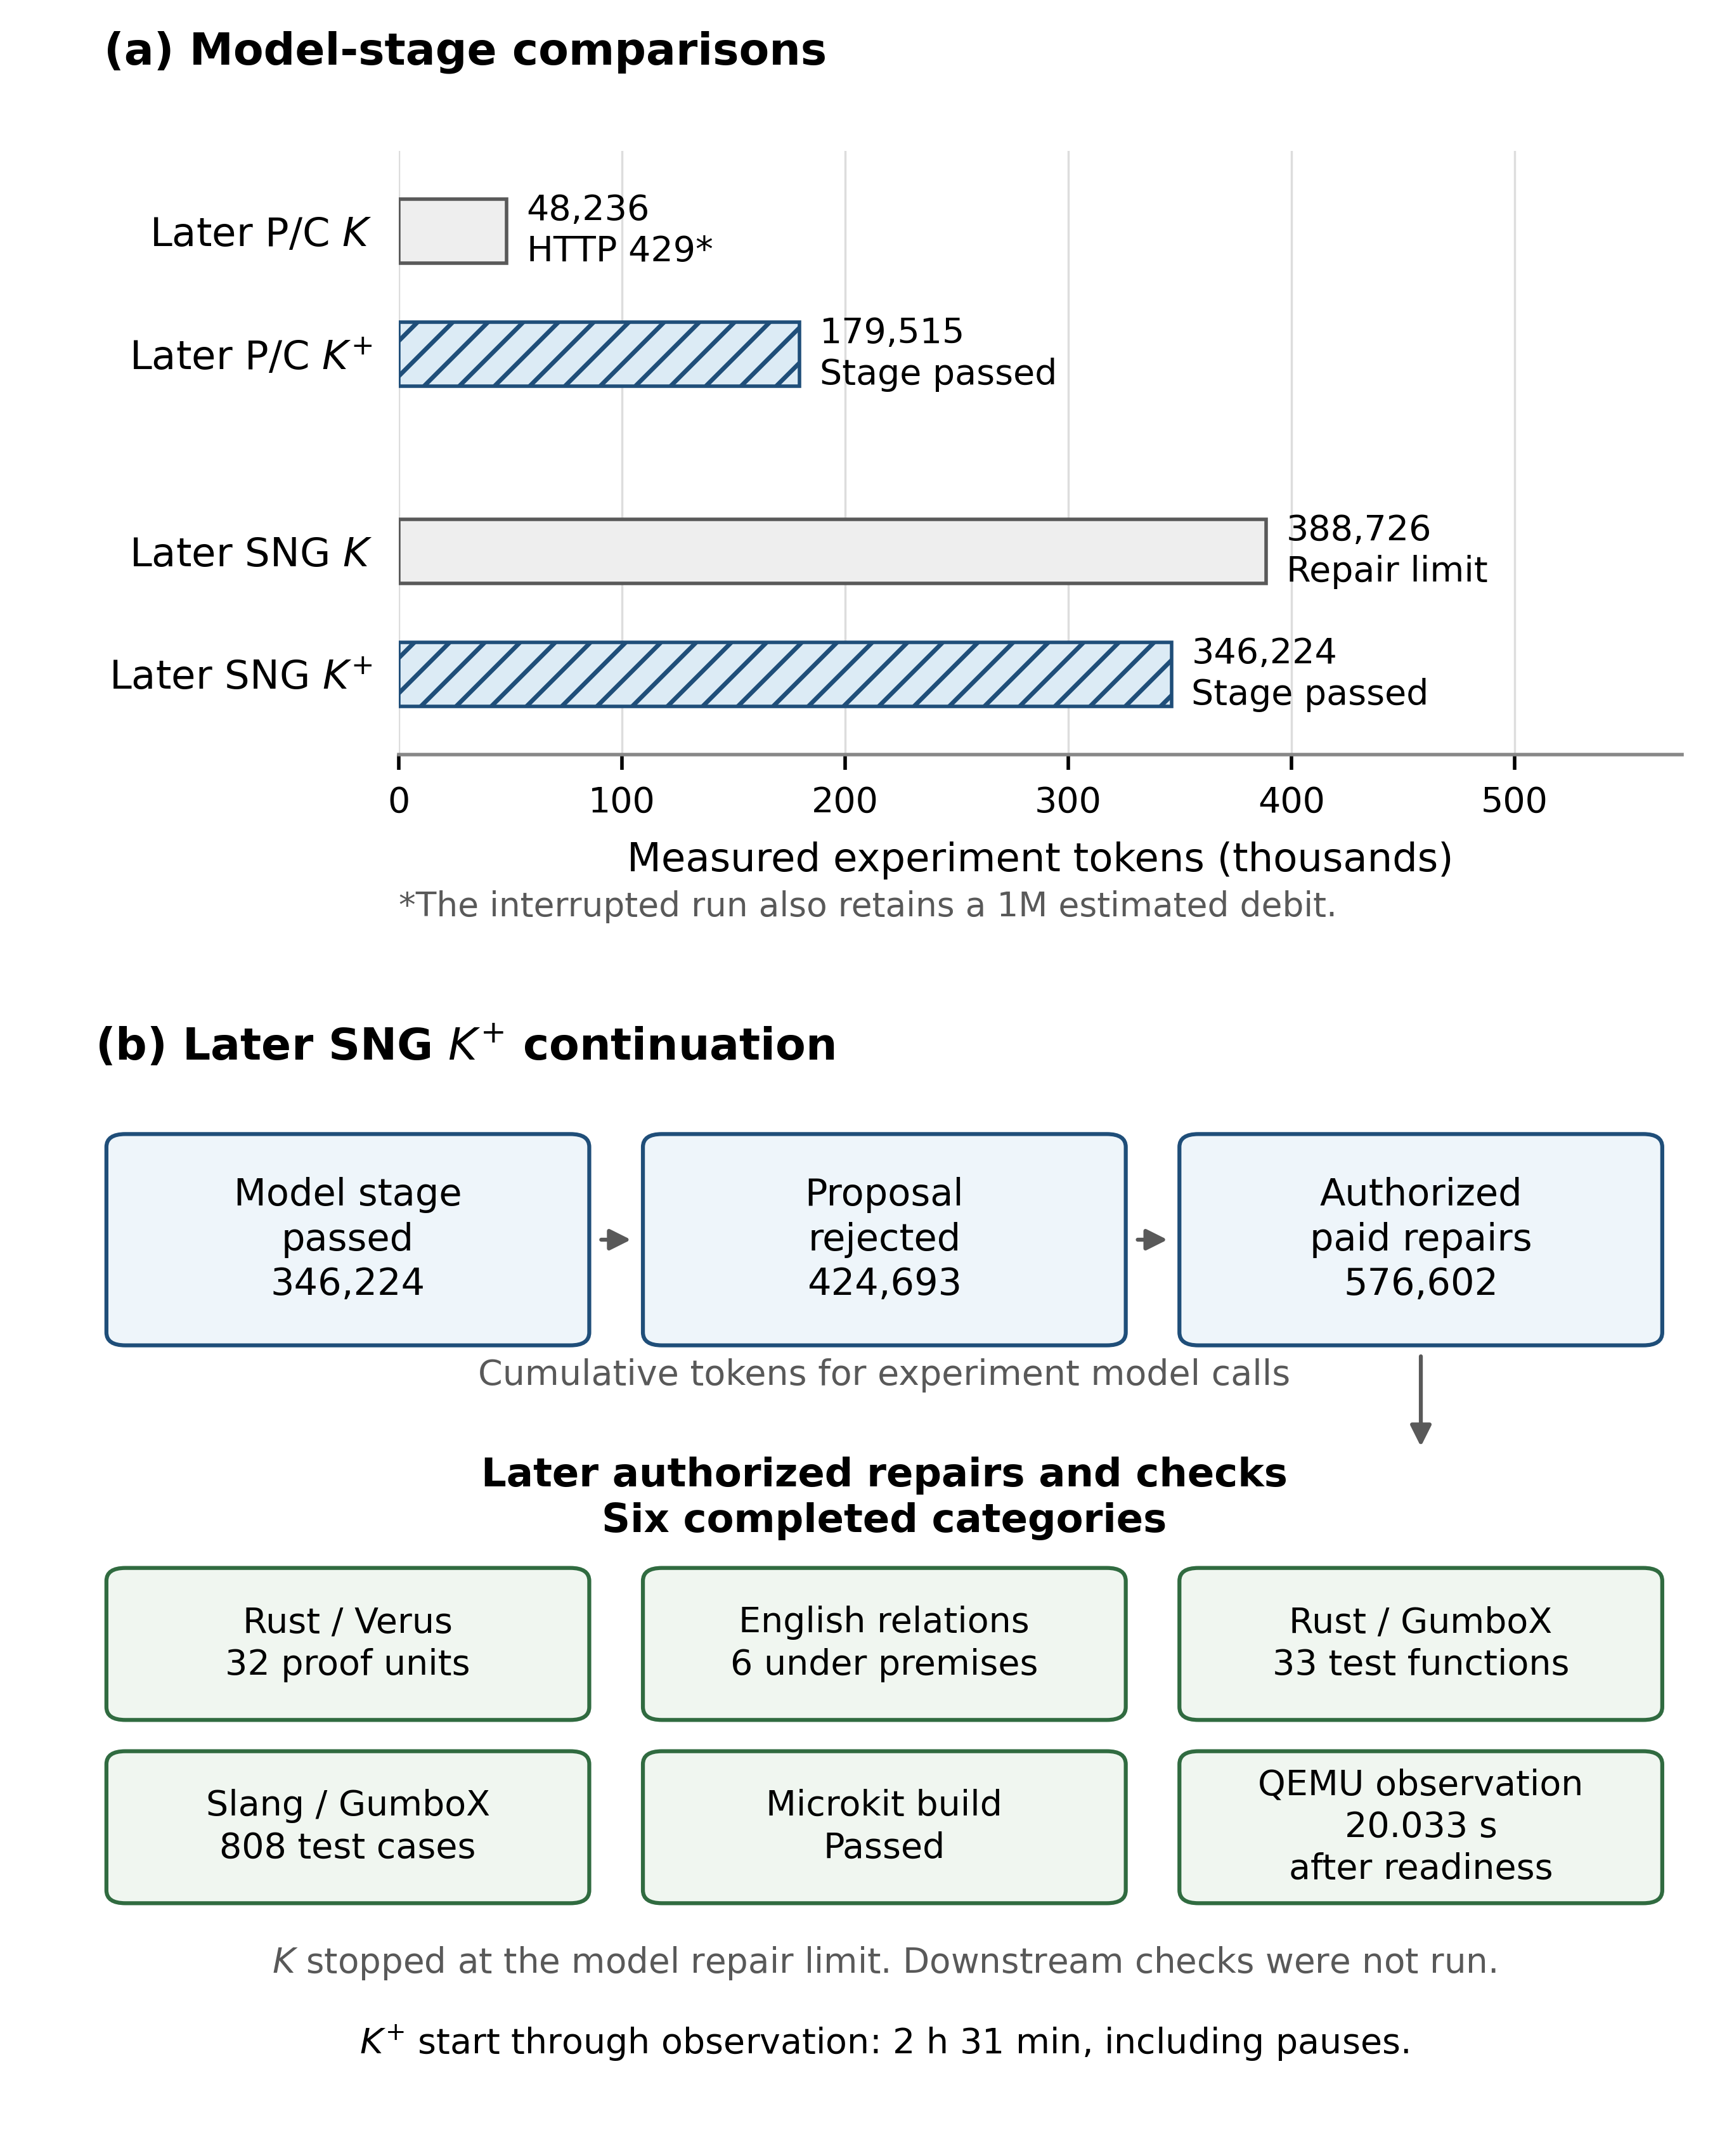
\includegraphics[width=\linewidth]{assets/comparison-results.png}
\caption{Later model comparisons for Producer/Consumer (P/C) and SNG. Panel (a) shows measured tokens through each model outcome. Panel (b) follows the later SNG $K^{+}$ candidate through the rejected proposal, paid repairs, and final checks. Serializer and initialization repairs after the paid calls add no measured experiment-model tokens. Appendix~\ref{app:evaluation-details} reports the first SNG construction separately.}
\Description{Four bars show the later Producer/Consumer K at 48236 measured tokens with HTTP 429, K plus at 179515 with one completed model target, later SNG K at 388726 at its repair limit, and later SNG K plus at 346224 with one completed model target. The continued K plus candidate used 576602 experiment-model tokens. The later SNG baseline's downstream checks were not run.}
\label{fig:comparison-results}
\end{figure}

